\documentclass[12pt, a4paper]{article}

% ------------------------------ font
\usepackage{times} %pdflatex
% \usepackage{luatexja}
% \usepackage{luatexja-fontspec}

% \setmainfont{Times New Roman}
% \setmainjfont[BoldFont=IPAexGothic]{IPAexMincho}
\usepackage{color}
\newcommand{\revise}[1]{{\color{red}{#1}}}

% ------------------------------ math
\usepackage{amsmath,amssymb}
\usepackage{siunitx}

% ------------------------------ author & natbib
\usepackage{authblk}
\renewcommand\Affilfont{\small}
\usepackage[semicolon]{natbib}
\bibliographystyle{elsarticle-harv.bst}

% ------------------------------ appendix
\usepackage[title]{appendix}

% ------------------------------ tables
\usepackage{here}
\usepackage{longtable, booktabs, array}
\usepackage{threeparttable, threeparttablex, multirow}
% \newcolumntype{d}{S[input-symbols = ()]}
\usepackage{lscape}

% ------------------------------- figures
\usepackage[labelfont=bf, labelsep=period, justification=justified]{caption}
\usepackage{graphics, graphicx}
\makeatletter
\def\maxwidth{\ifdim\Gin@nat@width>\linewidth\linewidth\else\Gin@nat@width\fi}
\def\maxheight{\ifdim\Gin@nat@height>\textheight\textheight\else\Gin@nat@height\fi}
\makeatother
% Scale images if necessary, so that they will not overflow the page
% margins by default, and it is still possible to overwrite the defaults
% using explicit options in \includegraphics[width, height, ...]{}
\setkeys{Gin}{width=\maxwidth,height=\maxheight,keepaspectratio}

% ------------------------------ page settings
\usepackage[left=3cm,right=3cm,top=3cm,bottom=3cm]{geometry}
\usepackage{setspace}
\renewcommand{\baselinestretch}{2}
\providecommand{\tightlist}{%
  \setlength{\itemsep}{0pt}\setlength{\parskip}{0pt}}

% ------------------------------ hyperlink
\usepackage[hidelinks]{hyperref}

% ------------------------------ other packages
\usepackage{booktabs}
\usepackage{siunitx}

  \newcolumntype{d}{S[
    input-open-uncertainty=,
    input-close-uncertainty=,
    parse-numbers = false,
    table-align-text-pre=false,
    table-align-text-post=false
  ]}
  

% ------------------------------ paper information
\title{Exploring Information Provision to Promote Stem Cell Donation:
Evidence from a Field Experiment of the Japan Marrow Donor Program}
\author[a]{%
  Hiroki Kato\thanks{Corresponding author. E-mail address: \href{mailto:hkato.econ@aoyamagakuin.jp}{\nolinkurl{hkato.econ@aoyamagakuin.jp}}}
}
\author[b]{%
  Fumio Ohtake\thanks{E-mail address: \href{mailto:ohtake@cider.osaka-u.ac.jp}{\nolinkurl{ohtake@cider.osaka-u.ac.jp}}}
}
\author[c]{%
  Saiko Kurosawa\thanks{E-mail address: \href{mailto:skurosaw@inahp.jp}{\nolinkurl{skurosaw@inahp.jp}}}
}
\author[d]{%
  Kazuhiro Yoshiuchi\thanks{E-mail address: \href{mailto:kyoshiuc-tky@umin.ac.jp}{\nolinkurl{kyoshiuc-tky@umin.ac.jp}}}
}
\author[e]{%
  Takahiro Fukuda\thanks{E-mail address: \href{mailto:tafukuda@ncc.go.jp}{\nolinkurl{tafukuda@ncc.go.jp}}}
}
\affil[a]{School of International Politics, Economics and Communication, Aoyama Gakuin University, 4-4-25 Shibuya, Shibuya-ku, Tokyo 150-8366, Japan}
\affil[b]{Center for Infectious Disease Education and Research (CiDER), Osaka University, 1-10 Yamadaoka, Suita, Osaka 565-0871, Japan\hspace{0pt}}
\affil[c]{Department of Oncology, Ina Central Hospital, 1313-1, Koshirokubo, Ina, Nagano 396-8555, Japan}
\affil[d]{Graduate School of Medicine, The University of Tokyo, 7-3-1 Hongo, Bunkyo, Tokyo 113-8655, Japan}
\affil[e]{Department of Hematopoietic Stem Cell Transplantation, National Cancer Center Hospital, 5-1-1 Tsukiji, Chuo-ku, Tokyo 104-0045, Japan}
\date{}

\makeatletter
\renewcommand*{\@fnsymbol}[1]{\ifcase#1\or*\else\@arabic{\numexpr#1-1\relax}\fi}
\makeatother

\begin{document}
\begin{spacing}{1}
  \maketitle
    \clearpage
  \begin{abstract}
  Allogeneic hematopoietic stem cell transplantation faces supply shortages, similar to the issue faced by organ transplantation. While many studies examine interventions that aim to increase donor registrations for organ transplantation from deceased donors, stem cell transplantation involves living donors, who may refuse to donate when matched with patients. Therefore, preventing such donor \revise{dropout} is crucial. Indeed, many transplant coordinations are interrupted before stem cells from donors can be collected. To address this issue, we developed a behavioral intervention in collaboration with the Japan Marrow Donor Program, which comprised adding messages based on insights from behavioral economics into the letters sent when donors are matched with patients. We then conducted a field experiment to verify the effect of our intervention. The results demonstrate that behavioral interventions bridging information gaps can prevent registered donor \revise{dropout} and increase donor availability for transplantation. Specifically, the message explaining the limited number of compatible donors per patient increased the probability of donors completing the confirmatory typing stage (available donors from whom physicians can choose the optimal donor for transplantation) by 12\%.

  \vspace{0.5em}

  \noindent
  \textit{Keywords}: prosocial behavior, field experiment, free-riding, information provision, Japan Marrow Donor Program, stem cell transplantation

  \vspace{0.5em}

  \noindent
  \textit{JEL classification}: D64, D90, H41, I11
  \end{abstract}
  \end{spacing}



\setcounter{footnote}{0}

\clearpage

\hypertarget{intro}{%
\section{Introduction}\label{intro}}

Allogeneic hematopoietic stem cell transplantation (HSCT) faces supply shortages in many countries---similar to the issues faced by organ transplantation---and significant efforts are being made to increase supply in transplantation. Many studies have examined interventions to increase donor registrations, particularly in the context of organ transplantation from deceased donors \citep[for example,][]{Kessler2012}. However, unlike organ transplantation from deceased donors, stem cell transplantation involves living donors. Therefore, registered donors---when matched with patients---may still refuse to donate. Consequently, registries in some countries have implemented interventions aimed at preventing such donor \revise{dropout} \citep{Switzer2018, Haylock2024}. However, more needs to be done to develop interventions to mitigate donor \revise{dropout}. Thus, we conduct a field experiment in Japan and argue that behavioral interventions aimed at bridging information gaps can prevent registered donor \revise{dropout}.

HSCT has the lowest relapse rate among all treatments for leukemia and other blood cancers. In this treatment, (1) anticancer drugs or radiation are used to kill tumor cells and (2) healthy hematopoietic stem cells are transplanted from a donor. The transplantation requires that the donor's white blood cell type (HLA) completely or partially matches the patient's HLA. While the probability of a complete match between two randomly selected individuals is less than 1\%, the probability of a full match between siblings is 30\%. In other words, potential donors who meet the transplantation requirements are more likely to be found among relatives. Therefore, in Japan, patients first search for donors among their relatives and, if no match is found, then seek unrelated donors through the \revise{Japan Marrow Donor Program} (JMDP).\footnote{When HLA-identical or partially matched unrelated donors are unavailable, several options exist. The first option is haploidentical stem cell transplantation in which stem cells are transplanted from a close relative with semi-matched HLA. The second option is cord blood transplantation in which stem cells are transplanted from the umbilical cord or placenta of pregnant women. The HLA requirements for these transplants are weaker than those for bone marrow (or peripheral blood stem cell (PBSC)) transplants between unrelated individuals. Notably, in Japan, bone marrow and PBSC transplants between unrelated individuals accounted for 20\% of all transplants in 2021 \citep{JapaneseDataCenterf2022}.}

However, only about half of the patients registered with the JMDP can receive transplantation because it takes time to confirm donors' intentions and ensure the safety of the transplantation. According to \citet{Hirakawa2018}, the median length of the transplantation process through the JMDP was 146 days (approximately five months), whereas 58\% of patients who died (or had their transplantation interrupted because of poor health) passed away within 200 days in 2004--2013. As a result, only 60\% of registered patients typically receive transplantation from unrelated donors through the JMDP. Therefore, the crucial goals of the JMDP are to both reduce the time to transplantation and increase the transplantation rate for registered patients.

Preventing registered donor \revise{dropout} is more important than increasing the number of registered donors to increase the transplantation rate. In Japan, most patients can eventually find donor candidates \citep{Takanashi2016}. Therefore, the marginal benefit of expanding the donor pool is small. However, most stem cell transplantation coordinations do not reach actual transplantation because, as noted earlier, registered donors may refuse to donate when they are matched with patients. Indeed, \citet{Hirakawa2018} reported that over half of transplant coordinations (56\%) did not reach confirmatory typing (CT) because of donor-related reasons. Since physicians select donors from candidates who undergo CT, donor \revise{dropout} before the CT stage reduces donor availability and can extend the time to transplantation. This problem occurs not only at the JMDP but also at other registries \citep[for example,][]{Balassa2019, Hamed2023, Haylock2024}. Thus, registries should explore and adopt interventions to increase the number of donor candidates who reach CT, thereby improving donor availability, while maintaining individuals' autonomy.

In this study, we develop a behavioral intervention to prevent registered donor \revise{dropout}, that is, increase the number of donor candidates who progress to the CT stage, in collaboration with the JMDP. The intervention adds messages based on insights from behavioral economics into the letters sent when donors are matched with patients. This letter informs matched donors that they are compatible with a specific patient requiring HSCT owing to their matching HLA and requests their participation in the transplantation coordination process. Upon responding to this so-called ``HLA match letter,'' matched donors indicate their willingness to donate and proceed to the next coordination stage, namely, the CT stage. In collaboration with the JMDP, we conduct a field experiment to examine the effect of our intervention on progressing the CT stage. Our field experiment includes 11,154 matched donors who received HLA match letters between September 2021 and February 2022.

The first message (the \emph{\revise{matching difficulty}} message) informs matched donors that the number of HLA-compatible donors per patient is limited. Stem cell donations are interchangeable if other potential donors in the registry have identical HLA types. Therefore, transplantation through the JMDP represents a public good facing the classic free-rider problem \citep{Bergstrom2009}. This message emphasizes the scarcity of compatible donors and aims to mitigate the lack of motivation associated with free-riding behavior.

The second message (the \emph{early coordination} message) informs matched donors that early coordination would increase the patient's transplantation rate. Our preliminary survey found that among registrants, those who placed higher value on immediate outcomes were more likely to proceed with donations \citep{Ohtake2020}. Motivated by this result, the early coordination message emphasizes the value of responding now, rather than postponing responses.

Using coordination data provided by the JMDP, we demonstrate that our intervention increases the probability of donors reaching the CT stage. Specifically, the \revise{matching difficulty} message increases the likelihood of donors reaching CT by 12\%. A back-of-the-envelope calculation suggests that this positive effect may partially mitigate the negative impact of the shrinkage of the future donor pool due to aging (as discussed in Section \ref{conclusion}). The \revise{matching difficulty} message primarily influences men with prior coordination experience. However, the early coordination message does not have the intended effect of encouraging early responses or increase the probability of donors reaching the CT stage. Our field experiment suggests that messages addressing information gaps regarding patient compatibility can prevent donor \revise{dropout}.

This study relates to the series of intervention studies in the context of transplantation. Previous research, primarily in economics and marketing, has focused on organ transplantation from deceased donors and developed interventions to increase the number of registrants. Since donors cannot receive monetary or material incentives from transplantation, self-interested individuals do not register as donors. To address this issue, previous studies have examined systems that grant priority rights to receive transplants as patients \citep{Kessler2012, Li2013, Stoler2017}.\footnote{When extending to organ transplantation from living donors, paid leave policy serves as an indirect financial incentive. \citet{Lacetera2014} examined the effects of this policy on organ donations from both living and deceased donors as well as stem cell transplantation.} In the absence of such incentives, donor registration depends on individual altruism. This is also true for stem cell transplantation \citep{Bergstrom2009, Ohtake2020}. In the context of organ transplantation from deceased donors, \citet{Sallis2018} and \citet{Robitaille2021} argued for the effectiveness of messages that stimulate altruistic motivations. Our research examines similar interventions.

However, unlike message intervention studies for organ transplantation from deceased donors, our policy goal is to prevent registrants from dropping out. As discussed above, registries should consider not only increasing registrants but also preventing registrant \revise{dropout} because registered donors may refuse to donate when matched with a patient. Medical research has long examined the factors driving registered donor \revise{dropout} \citep{Switzer2003, Switzer2004, Balassa2019, Hamed2023}. Additionally, several recent studies have examined the effectiveness of measures to prevent such \revise{dropout} \citep{Switzer2018, Haylock2024}. In particular, \citet{Switzer2018} pointed out the importance of providing accurate information on compatibility with patients. The first of our intervention messages (the \revise{matching difficulty} message) is similar to what \citet{Switzer2018} advocated. To the best of our knowledge, we conduct the first randomized controlled trial to verify measures to prevent donor \revise{dropout} in the context of stem cell transplantation. Our findings provide practical insights to marrow donor programs worldwide.

Finally, our research makes significant contributions to the broader context. Previous studies have examined the effects of behavioral interventions such as message and information provision in health and medical policy contexts, including vaccination \citep[for example,][]{Dai2021, Milkman2021}, breast cancer screening \citep{Bertoni2020}, and cord blood transplantation \citep{Grieco2018}. From the perspective of the target population for interventions, there is an important difference between interventions in these contexts (including organ transplantation from deceased donors) and our intervention. The former interventions target the general population. By contrast, our intervention targets a subset of the general population (i.e., registered donors). This difference results in significant differences in the preferences of the target population. While the general population includes individuals with various preferences, our target population includes many altruistic individuals, who tend to be more likely to register as stem cell donors \citep{Bergstrom2009, Ohtake2020}. As we develop interventions targeting a population skewed toward altruistic individuals, whether previous findings apply to our case is uncertain and the intervention effects need to be verified appropriately. As a result of our experiment, we argue that illuminating messages that bridge information gaps can be effective---even in a skewed population.

The remainder of this paper is organized as follows. Section \ref{experiment} provides an overview of the coordination process of the JMDP and describes our field experiment. Section \ref{result} presents the results of our experiment. Section \ref{conclusion} discusses the results and concludes.

\hypertarget{experiment}{%
\section{Field Experiment}\label{experiment}}

\hypertarget{background}{%
\subsection{Background: Coordination Process of JMDP}\label{background}}

To allow readers to better understand our intervention and data, we first outline the coordination process leading to the donation of stem cells by donors registered with the JMDP. First, when a registrant is matched with a patient enrolled in the JMDP, the JMDP office sends the matched donor the HLA match letter.\footnote{Simultaneously, the JMDP office sends a social networking message to matched donors informing them that the JMDP has sent the HLA match letter.} In this letter, the JMDP recommends that the matched donor respond within seven days (see Table \ref{tab:list-message}). The matched donor completes a medical questionnaire and indicates their willingness to donate upon responding the letter. Matched donors who express a willingness to donate move onto the coordination process.

A matched and willing donor undergoes CT within approximately one month. CT confirms whether the matched donor meets the appropriate donor criteria set by the JMDP. The transplantation coordinator delegated by the JMDP explains the details of the donation process and asks matched donors and their families about their willingness to donate. Thereafter, the coordinating physician conducts medical interviews, examinations, and blood tests, including those for infectious disease markers. Collection methods (bone marrow or PBSC collection) are also determined based on the preferences of the matched donor and coordinating physician. CT can be skipped when a previous CT result remains valid.

Physicians can choose up to 10 potential donors to proceed to this stage simultaneously. Importantly, a matched donor cannot have access to any information about the matched patient (for example, the number of other available potential donors), nor can the potential donor obtain this information from the transplantation coordinator or coordinating physician. Physicians can select the most appropriate donor for transplantation from among the matched donors who undergo CT. Thus, it is important to increase the probability of donors reaching CT to increase the transplantation rates of registered patients.

The matched donor selected as the best donor must provide final consent after being informed of their selection by the coordinator and coordinating physician. Simultaneously, a representative of the donor's family must provide consent to the donation. After final consent is obtained, the selected donor cannot withdraw their decision to donate. They then undergo a surgical procedure to collect stem cells. The time from CT to collection is approximately three to four months.

\hypertarget{design}{%
\subsection{Experimental Design}\label{design}}

\begin{table}

\caption{\label{tab:list-message}List of Intervention Messages}
\centering
\fontsize{8}{10}\selectfont
\begin{threeparttable}
\begin{tabular}[t]{l>{\raggedright\arraybackslash}p{40em}}
\toprule
Message & Content\\
\midrule
Standard message & We inform you that your HLA type (white blood cell type) matches that of a patient in our registry, and you have been selected as one of our potential donors. We are contacting you to ask if you would like to undergo further testing and interviews in preparation for donation. Please read the enclosed materials carefully, consider whether coordination is possible, and return the form within seven days of receiving this information. [\emph{Insert intervention messages here}] If we proceed with coordination after receiving your return, a coordinator will contact you by phone to discuss the details of your request.\\
\addlinespace[0.3em]
\multicolumn{2}{l}{\textbf{Intervention message}}\\
\hspace{1em}\revise{Matching difficulty} message & The number of registered donors whose HLA type matches that of a single registered patient is one in hundreds to tens of thousands. We hope you understand that while we may find more than one potential donor, it will not be a large number.\\
\hspace{1em}Early coordination message & Approximately 60\% of patients receive a transplant through the JMDP. The earlier a donor can be found to donate bone marrow, the greater the probability of the patient receiving a transplant.\\
\bottomrule
\end{tabular}
\begin{tablenotes}
\item \emph{Note}: Translated by the authors.
\end{tablenotes}
\end{threeparttable}
\end{table}

Our intervention involved adding two messages into the HLA match letter.\footnote{In designing our intervention messages, we were careful to avoid placing undue psychological pressure on potential donors. Specifically, we avoided using language that sounded like an appeal. Additionally, we only used information publicly available from the JMDP. Finally, the risks of transplantation were explained in a typical manner. The intervention message was approved by the institutional review boards of the Graduate School of Economics, Osaka University and the JMDP.} Table \ref{tab:list-message} lists the content of the standard letter and the two intervention messages. The JMDP also encloses a handbook that describes the coordination process as well as the medical questionnaire and donor consent form.\footnote{The handbook can be found at \url{https://www.jmdp.or.jp/pdf/en/DonorHandBook201708.pdf} (Accessed December 9, 2024).}

The \revise{matching difficulty} message emphasizes the low number of matched donors per registered patient. If other potential donors with the same HLA type are in the pool, one donor's donation can be substituted with that of another compatible donor. Additionally, multiple matched donors (up to 10) can be simultaneously matched with a single patient. Therefore, transplantation through the JMDP faces the classical free-rider problem \citep{Bergstrom2009}. Additionally, \citet{Kurosawa2022} interviewed previously matched donors and found that those with low donation intention felt that they were ``one of several donors.'' This implies that some potential donors with low intention recognize that their donation could be substituted by others. Because the \revise{matching difficulty} message emphasizes the small number of possible substitutes, this message is expected to discourage free-riding and increase the willingness to donate.\footnote{Alternatively, the \revise{matching difficulty} message makes the rarity of the opportunity to donate more salient, which may change donor behavior.}

The early coordination message emphasizes that early coordination would increase the patient's transplantation rate. Our preliminary survey found that registered donors who place higher value on immediate outcomes were more likely to proceed with donations \citep{Ohtake2020}. Motivated by this finding, we created a message that emphasized the value of responding now, rather than postponing the response. Furthermore, earlier responses are associated with higher rates of reaching the CT stage (see Figure A1 in Supplementary Material A). Therefore, this message is expected to increase the probability of donors undergoing CT.

Four experimental groups were established to estimate the effects of including the two intervention messages. First group received the standard HLA match letter with neither of the intervention messages, serving as a control group (\revise{StatusQuo} group). Second and third group received the standard HLA match letter including only the probability and early coordination messages, respectively (\revise{MatchMessage} group and \revise{CoordMessage} group, respectively). The last group received the standard HLA match letter with both intervention messages included to test the negative effect of information overload (\revise{BothMessage} group).

The participants in the experiment were 11,154 matched donors who received HLA match letters between September 6, 2021 and February 27, 2022. To maintain randomness to the best of the JMDP office's abilities, we assigned the participants to the four experimental groups using weekly cluster randomization. Specifically, we created a cluster every seven days (a week starting from Monday) and randomly assigned one experimental group to each cluster (see Table A1 in Supplementary Material A for the assignment schedule).\footnote{The experiment was not conducted from December 27, 2021 to January 3, 2022 because the JMDP was closed for the New Year's holiday.} The assignment of the experimental groups was designed to be as balanced across weeks and months as possible. Before conducting the experiment, we obtained approval from the institutional review boards of the Graduate School of Economics, Osaka University (approval number: R030305) and the JMDP (approval number: JMDP2021-04).

\hypertarget{data-and-empirical-strategy}{%
\subsection{Data and Empirical Strategy}\label{data-and-empirical-strategy}}

In the coordination data provided by the JMDP, the unit of observation was the matched donors. The data included individual characteristics such as the donor's sex, age, number of coordination experiences, and prefecture-level residential area. The data on the coordination process included whether each stage (response to the letter, CT, donor selection, final consent, and collection) had been completed. Additionally, the data included the number of days taken to respond and willingness to donate. If the coordination process was interrupted, the reasons for the interruption were recorded in three categories (patient-side, donor non-health, and donor health reasons). The analysis included 11,049 matched donors living in Japan whose coordination process was completed or interrupted.\footnote{One matched donor lived abroad. There were 104 matched donors with ongoing coordination at the time of data collection. The proportion of matched donors with ongoing matching was balanced across the experimental groups (F-test, p-value = \(0.383\)).}

The primary outcome was whether matched donors underwent CT. Responses that did not confirm a willingness to donate and late responses lead to coordination interruptions before the CT stage. Moreover, as physicians can select the most appropriate donor for transplantation from among the matched donors who have undergone CT, showing up for CT represents a costly prosocial behavior, including response behavior, as well as an important practical indicator.

As additional data, we used the list of medical institutions published on the JMDP website.\footnote{\url{https://www.jmdp.or.jp/hospitals/view2/} (Accessed August 4, 2022).} This list includes complete addresses, the availability of bone marrow collection, and the availability of PBSC collection. We aggregated this list at the prefecture level, calculated the number of hospitals per 10 square kilometers, and merged the results with the coordination data using the prefecture as the merge key. We considered this variable as the traveling cost of coordination and donation.

\begin{table}

\caption{\label{tab:summary}Summary of the Field Experiment}
\centering
\fontsize{8}{10}\selectfont
\begin{threeparttable}
\begin{tabular}[t]{lccccc}
\toprule
\multicolumn{1}{c}{ } & \multicolumn{4}{c}{Experimental Groups} & \multicolumn{1}{c}{ } \\
\cmidrule(l{3pt}r{3pt}){2-5}
 & StatusQuo & MatchMessage & CoordMessage & BothMessage & F-test, p-value\\
\midrule
\addlinespace[0.3em]
\multicolumn{6}{l}{\textbf{A. Interventions}}\\
\hspace{1em}Standard message & X & X & X & X & \\
\hspace{1em}\revise{Matching difficulty} message &  & X &  & X & \\
\hspace{1em}Early coordination message &  &  & X & X & \\
\addlinespace[0.3em]
\multicolumn{6}{l}{\textbf{B. Sample Size}}\\
\hspace{1em}N & 2535 & 3053 & 2726 & 2735 & \\
\addlinespace[0.3em]
\multicolumn{6}{l}{\textbf{C. Balance Test}}\\
\hspace{1em}Male (= 1) & 0.624 & 0.633 & 0.631 & 0.609 & 0.231\\
\hspace{1em}Age & 38.376 & 38.121 & 37.448 & 37.978 & 0.004\\
\hspace{1em}Number of past coordinations & 1.609 & 1.589 & 1.625 & 1.563 & 0.130\\
\hspace{1em}Number of listed hospitals & 0.476 & 0.490 & 0.487 & 0.485 & 0.835\\
\hspace{1em}Number of hospitals listed with PBSC collection & 0.162 & 0.167 & 0.166 & 0.164 & 0.838\\
\hspace{1em}Number of hospitals listed with BM collection & 0.246 & 0.256 & 0.254 & 0.251 & 0.741\\
\hspace{1em}Number of holidays & 4.544 & 5.828 & 4.466 & 4.770 & 0.000\\
\hspace{1em}Skipped CT (= 1) & 0.039 & 0.047 & 0.046 & 0.050 & 0.233\\
\bottomrule
\end{tabular}
\begin{tablenotes}
\item \emph{Note}: For the balance test, we regressed a covariate on treatment dummies and tested the null hypothesis that all coefficients are zero. We used robust standard errors for the statistical inference. Abbreviation: PBSC = peripheral blood stem cell; BM = bone marrow.
\end{tablenotes}
\end{threeparttable}
\end{table}

Table \ref{tab:summary} summarizes our experiment. Panels A and B present the intervention and sample size for each experimental group, respectively. Panel C presents a balance test of whether the randomization was successful. There were statistically significant differences in the average age and number of holidays in the assigned and following weeks between the experimental groups.\footnote{Although cases eligible for skipping CT were balanced across all the experimental groups, there was an imbalance between \revise{the BothMessage group} and the \revise{StatusQuo} group (see Table A3 in Supplementary Material A). This imbalance becomes an important factor in interpreting the effect of \revise{the BothMessage group}.} The average age of \revise{the CoordMessage group} was approximately one year younger than that of the \revise{StatusQuo} group. However, this difference was negligible from a standardized mean difference perspective (see Table A2 in Supplementary Material A). The average number of holidays for \revise{the MatchMessage group} was higher than that of the \revise{StatusQuo} group. This occurred because the week following the week in which \revise{the MatchMessage group} was assigned in December included the New Year's holiday (see Table A1 in Supplementary Material A).\footnote{In Japan, the New Year's holiday is set by the government to run from December 29 to January 3. While we follow this definition, this holiday may be extended depending on individual circumstances.}

Although most covariates were balanced across the experimental groups, a few covariates were unbalanced. Therefore, in addition to a simple difference of means test, we estimated the following linear regression model for individual \(i\) who received the HLA match letter in week \(w\):

\begin{equation}
  \begin{split}
  Y_{iw} =& \alpha + \beta_1 \cdot \text{MatchMessage}_{w}
  + \beta_2 \cdot \text{CoordMessage}_{w} + \beta_3 \cdot \text{BothMessage}_{w} \\
  &+ X'_{iw} \gamma + u_{iw},
  \end{split}\label{eq:reg}
\end{equation}

\noindent
where \(X_{iw}\) is a vector of the individual characteristics, including age and the number of holidays. The parameters of interest are \((\beta_1, \beta_2, \beta_3)\). \revise{We used standard errors clustered by the assigned week for statistical inference because all donors who matched with the same patient might receive the letter in the same week.}

\hypertarget{result}{%
\section{Experimental Results}\label{result}}

\hypertarget{main}{%
\subsection{Average Treatment Effects on CT}\label{main}}

Estimating the effect of the intervention messages on reaching the CT stage is critical because physicians select the optimal donor for transplantation from among matched donors who have undergone CT. We used a dummy variable coded one if a matched donor reached the CT stage.\footnote{We also coded the CT dummy one if CT was skipped.} In the \revise{StatusQuo} group, only \(22.25\)\% of matched donors underwent CT.

There are two reasons for the low probability of reaching CT. First, only \(54.91\)\% of the donors in the \revise{StatusQuo} group indicated their willingness to donate. Second, only \(40.52\)\% of those who expressed a willingness to donate reached the CT stage. Most \revise{dropout} between the response and CT stages occurred because of donor-related reasons (\(85.99\)\%). \citet{Hirakawa2018} found similar results and showed that the top three donor-related reasons were health issues, scheduling conflicts, and the lack of family consent. Our intervention messages are expected to increase the probability of reaching CT by both improving the willingness to donate and preventing dropouts between the response and CT stages.

\begin{figure}[t]
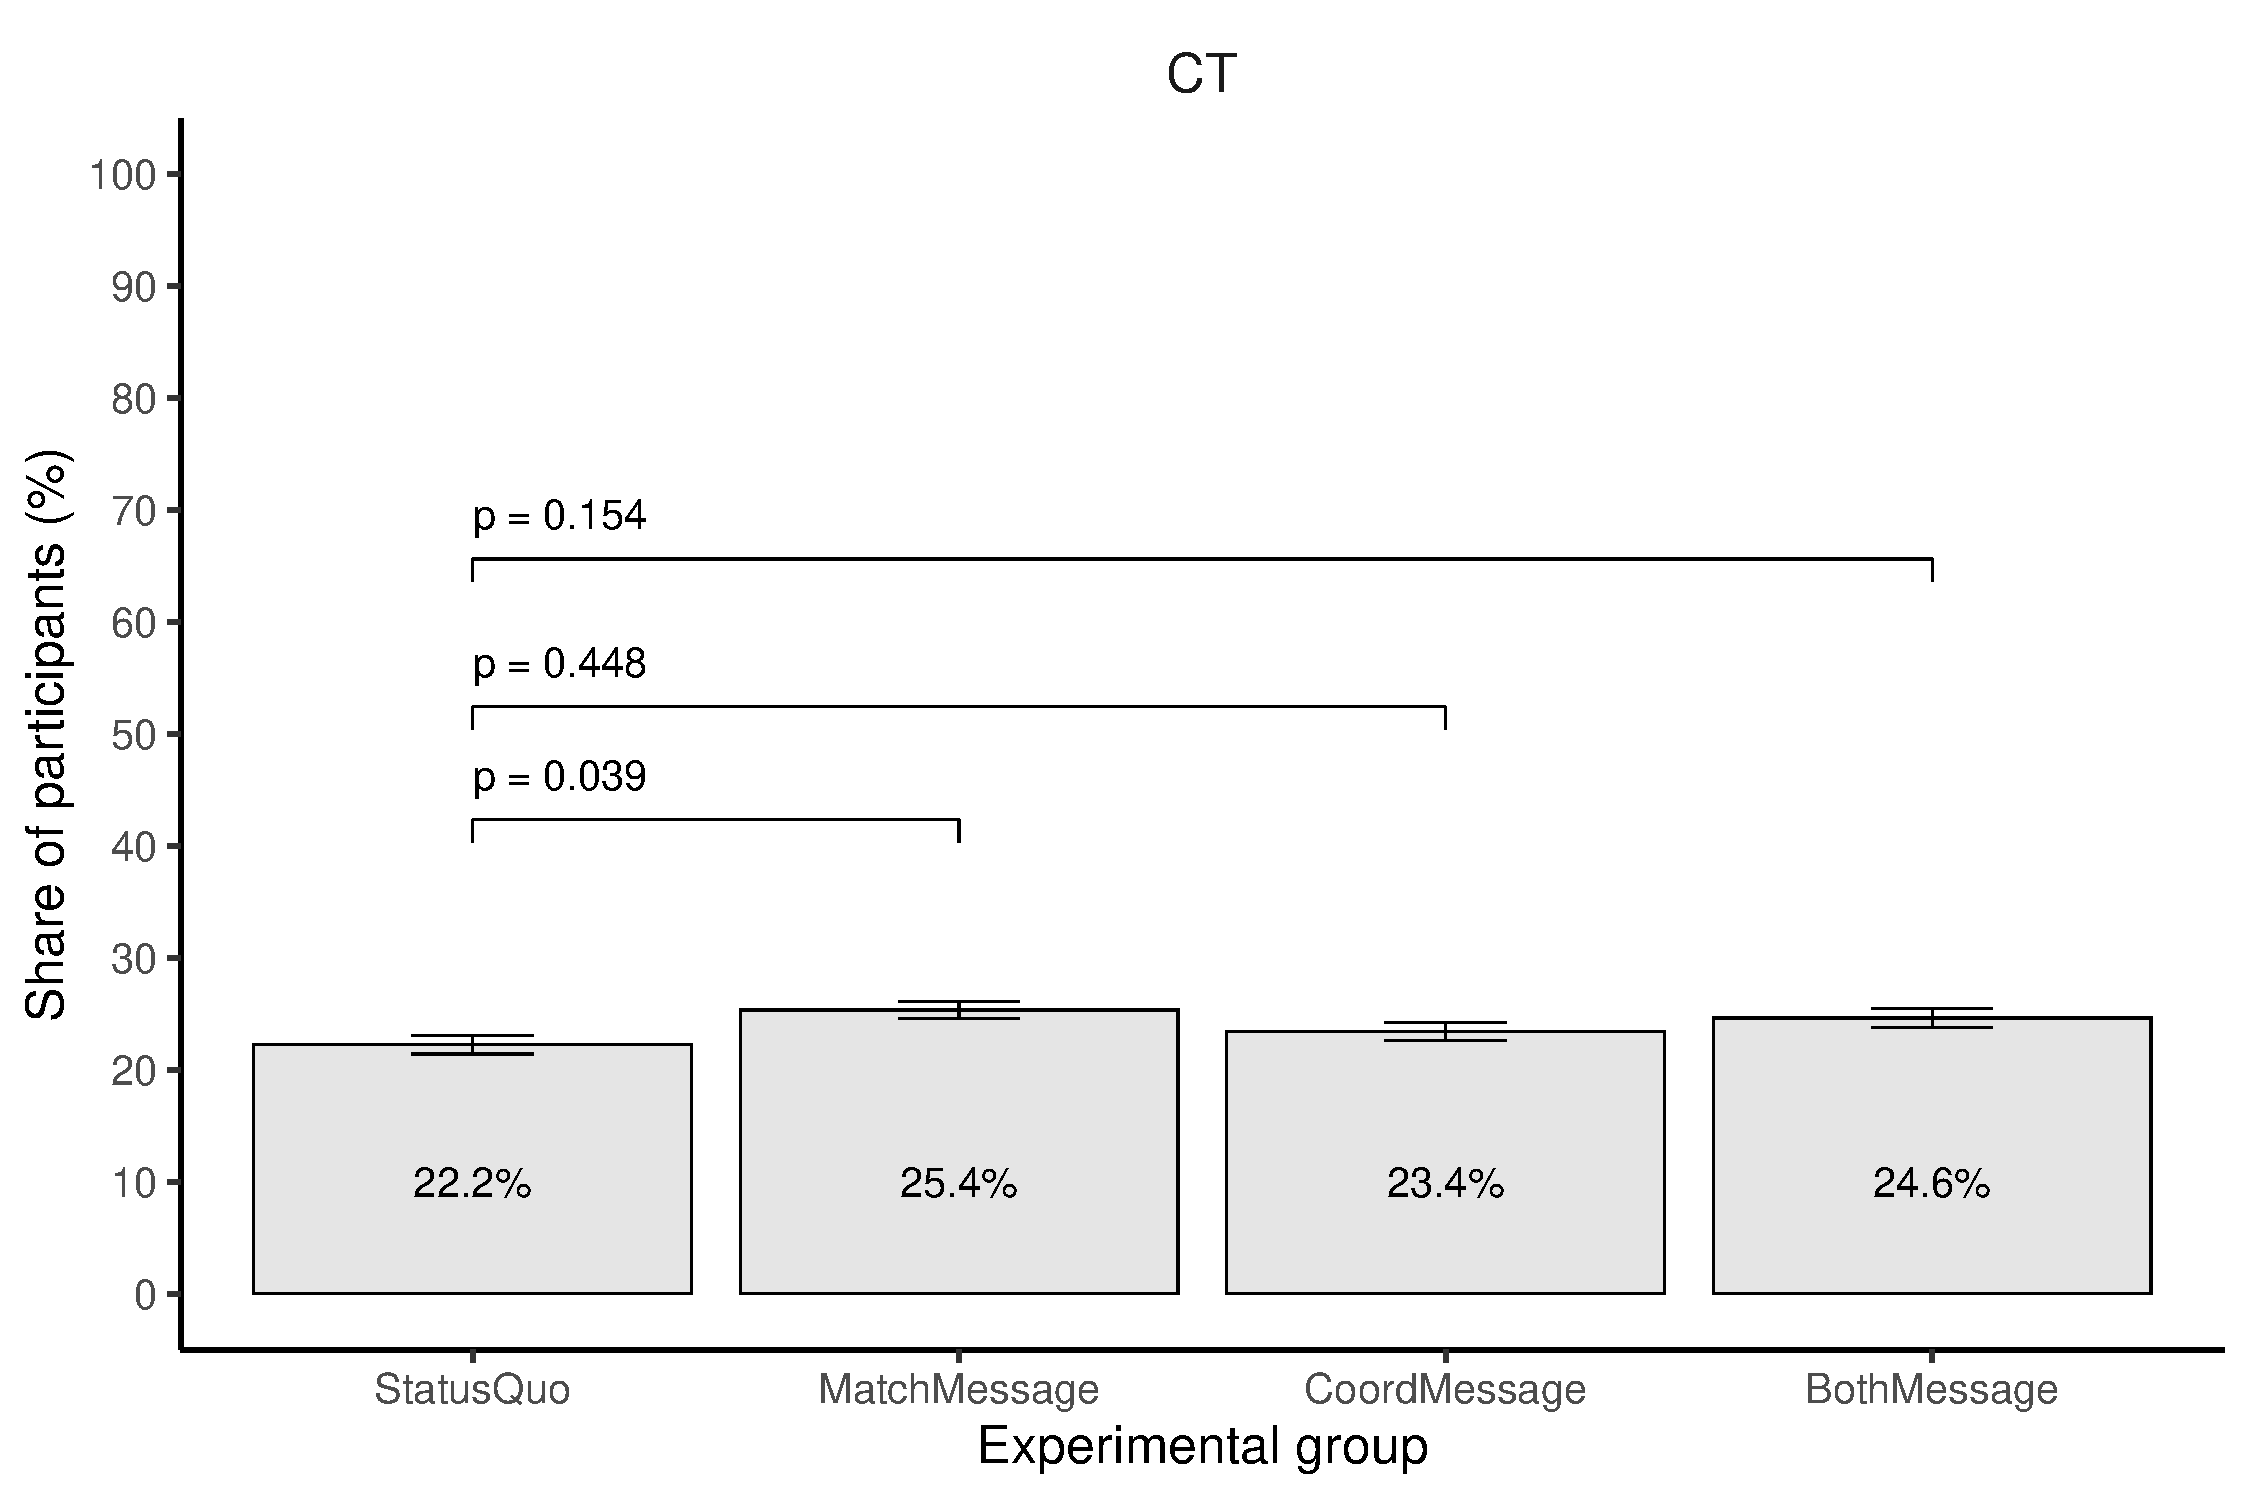
\includegraphics{JMDPRC~1/figure-latex/test-diff-mean-1} \caption{Sample Proportion of Reaching CT by Experimental Groups.\newline \emph{Note}: Error bars show standard errors of the mean. For the statistical test, we used standard errors clustered by the assigned week.}\label{fig:test-diff-mean}
\end{figure}

The proportions of donors reaching the CT stage for each of the experimental groups are presented in Figure \ref{fig:test-diff-mean}. \revise{Experimental groups B, which received the matching difficulty message, had a $3.1$ percentage point higher probability of reaching CT than the \revise{StatusQuo} group. This effect was} statistically significant. We obtained the same results when we adjusted for multiple \revise{hypotheses} testing, as proposed by \citet{List2019} (see Column (1) of \revise{Table A4 in Supplementary Material A}). The effect of \revise{the MatchMessage group} remained statistically significant when controlling for the covariates \revise{month fixed effects} using a linear probability model (see Column (2) of \revise{Table A4 in Supplementary Material A}). \revise{Also, this result was} robust to using logistic regression models instead of linear probability models (see Table \revise{A5} in Supplementary Material A). In summary, the \revise{matching difficulty} message included in the HLA match letter sent to \revise{the MatchMessage group} increased the probability of those participants reaching the CT stage.

\begin{table}

\caption{\label{tab:lm-test-decompose}Decomposition of Effect on the CT}
\centering
\fontsize{8}{10}\selectfont
\begin{threeparttable}
\begin{tabular}[t]{lcccccc}
\toprule
\multicolumn{1}{c}{ } & \multicolumn{3}{c}{Positive intention} & \multicolumn{3}{c}{No endogenous dropout} \\
\cmidrule(l{3pt}r{3pt}){2-4} \cmidrule(l{3pt}r{3pt}){5-7}
  & (1) & (2) & (3) & (4) & (5) & (6)\\
\midrule
MatchMessage group & \num{2.31}* & \num{1.86}* & \num{1.27} & \num{0.97} & \num{1.14} & \num{0.93}\\
 & (\num{1.33}) & (\num{1.07}) & (\num{0.93}) & (\num{1.02}) & (\num{1.09}) & (\num{0.92})\\
CoordMessage group & \num{-0.44} & \num{-0.05} & \num{-0.31} & \num{2.55}** & \num{1.50} & \num{1.46}\\
 & (\num{1.43}) & (\num{1.22}) & (\num{1.18}) & (\num{1.24}) & (\num{1.21}) & (\num{1.03})\\
BothMessage group & \num{0.59} & \num{0.24} & \num{0.12} & \num{2.27}** & \num{1.97}* & \num{1.92}*\\
 & (\num{1.61}) & (\num{1.37}) & (\num{1.09}) & (\num{1.04}) & (\num{1.14}) & (\num{1.04})\\
\midrule
Control average & 54.91 & 54.91 & 54.91 & 71.91 & 71.91 & 71.91\\
Covariates &  & X & X &  & X & X\\
Month FE &  &  & X &  &  & X\\
Num.Obs. & \num{11049} & \num{11049} & \num{11049} & \num{11049} & \num{11049} & \num{11049}\\
\bottomrule
\end{tabular}
\begin{tablenotes}
\item \emph{Note}: * $p < 0.1$, ** $p < 0.05$, *** $p < 0.01$. The robust standard errors are in parentheses. The unit of treatment effect is a percentage point. The outcome ``No endogenous dropout'' is a dummy variable that takes a value of 1 if coordination was not interrupted due to endogenous reasons (donor-side reasons) between reply with positive intention and CT. Covariates are gender, age, its squared term, the number of past coordinations, the number of public holidays in the assigned week and the following week, the number of hospitals per 10 square kilometers, the number of hospitals with PBSC collection per 10 square kilometers, the number of hospitals with BM collection per 10 square kilometers, and a dummy indicating that candidate can have skipped the CT. All covariates except gender dummy and dummy of skipped CT were demeaned.
\end{tablenotes}
\end{threeparttable}
\end{table}

As mentioned previously, our intervention was expected to increase the probability of reaching CT by improving the willingness to donate and preventing dropouts between the response and CT stages. Therefore, we decomposed the intervention message effects into three components: responses with a willingness to donate, prevention of \revise{dropout} because of patient-side reasons (exogenous \revise{dropout}), and prevention of \revise{dropout} because of donor-side reasons (endogenous \revise{dropout}). We call \revise{dropout} because of patient-side reasons ``exogenous \revise{dropout}'' because it occurs owing to factors outside donors' decision making. The results are presented in Table A5 in Supplementary Material A. The total effects on these three factors was equal to the overall message effect on completing CT. Although these effects were not statistically significant, after controlling for the covariates, the result suggested that the \revise{matching difficulty} message that increased the CT completion rate could have contributed to both improving and maintaining the willingness to donate. In particular, the \revise{matching difficulty} message contributed more to improving the willingness to donate, accounting for half of the effect on reaching CT.\footnote{We divided the effect of \revise{the MatchMessage group} on responses that included a willingness to donate by the sum of the absolute values of the effects on the three factors (\(3.44\) for \revise{the MatchMessage group}).}

The early coordination message included in the HLA letter sent to \revise{the CoordMessage group} was expected to increase the CT completion rate by encouraging early responses. Among donors who indicated a willingness to donate, those who responded earlier had a higher probability of reaching CT (see Figure A1 in Supplementary Material A). Therefore, we examined whether \revise{the CoordMessage group}, which did not show an overall increase in the willingness to donate, may have shown increased early responses accompanied by a willingness to donate. Figure A2 in Supplementary Material A presents the cumulative response rates of the willingness to donate over time for the experimental groups. Because the JMDP requests responses within seven days, we define early responses as cumulative response rates with a willingness to donate within seven days. However, the probability of responding with a willingness to donate within seven days did not increase in \revise{the CoordMessage group}. This result was also confirmed by the regression analysis (see Table A6 in Supplementary Material A). Therefore, the early coordination message did not have the expected effect.

\hypertarget{discussion}{%
\section{Discussion}\label{discussion}}

\hypertarget{conclusion}{%
\section{Conclusions}\label{conclusion}}

This study examined how information provision affects donor availability in stem cell transplantation. The results of our field experiment demonstrated that providing information on the limited number of HLA-compatible donors per patient (that is, the \revise{matching difficulty} message) increased the probability of reaching CT by enhancing and maintaining the willingness to donate. This result suggests that physicians can select optimal donors for transplantation from a larger pool of candidates. However, when presented simultaneously with an ineffective early coordination message, the positive effect of the \revise{matching difficulty} message was diminished. We speculate this is because of the negative effect of information overload. Therefore, it is important to convey effective information in a simple manner.

Although we cannot obtain robust evidence of heterogenous treatment effects, we suggest that the \revise{matching difficulty} message primarily affected men with prior coordination experience. Recent reviews have shown that when multiple donor options are available, physicians prefer male donors \citep{Fingrut2018} because patients with male donors are less likely to develop GVHD.\footnote{GVHD is a phenomenon in which donor-derived lymphocytes mistakenly identify the patient's normal cells as foreign and attack them, potentially leading to fever, skin symptoms, gastrointestinal symptoms such as diarrhea, and liver damage that may cause impaired consciousness.} Similar evidence has been obtained in Japan \citep{Shinohara2017}. Similarly, in our data, among matched donors who completed CT, male donors were more likely to be selected as transplant donors than female donors (see Table A10 in Supplementary Material A). Considering these facts and findings, the \revise{matching difficulty} message may improve coordination efficiency by promoting CT completion among male donors.

To evaluate the cost effectiveness of the intervention, we assess the impact of the \revise{matching difficulty} message on donor recruitment. The \revise{matching difficulty} message increased the CT completion rate by \(12\% (= 2.56/22.25)\). We can then calculate how many additional donor registrations would be needed to achieve this same 12\% increase in the CT completion rate. First, the positive effect of the \revise{matching difficulty} message on CT is equivalent to increasing the number of registered donors who match with patients by 12\%.\footnote{Let \(N_m\) be the number of registrants who start the coordination process. Let \(N_1(d)\) be the number of potential donors who reach CT under treatment \(d\). Then, \(N_1(d) = p(d)N_m\) holds, where \(p(d)\) is the probability of reaching CT under treatment \(d\). Note that \(d = 1\) and \(d = 0\) represent the treatment and control groups, respectively. We solve \(N_1(1) = p(0)[N_m + \Delta N_m]\) for \(\Delta N_m\), where \(\Delta N_m\) represents the increase in registrants who start coordination. Therefore, we obtain \([p(1) - p(0)]/p(0) = \Delta N_m/N_m\).} Since 40\% of registrants become matched donors, \(224,000\) of the current \(560,000\) registrants are potential matched donors.\footnote{The cumulative number of registrants since the JMDP's establishment is \(980,000\). Among these registrants, \(390,000\) have become potential donors who started the coordination process. Therefore, 40\% of registrants become potential donors who start coordination. Data source: \url{https://www.bs.jrc.or.jp/bmdc/donorregistrant/m2_03_00_statistics.html} (Accessed December 8, 2024).} Therefore, the effect of the \revise{matching difficulty} message on CT is equivalent to increasing the number of matched donors from \(224,000\) to \(250,000 (= 224,000 \times 1.12)\), an increase of \(26,000\). Alternatively, the effect of the \revise{matching difficulty} message on CT is equivalent to increasing the number of registrants from \(560,000\) to \(630,000 (= 560,000 \times 1.12)\), an increase of \(70,000\). The current JMDP donor pool includes \(100,000\) registered donors in their 50s.\footnote{\url{https://www.jmdp.or.jp/about/read/number/} (Accessed December 8, 2024).} Owing to the age limit for donation (54 years), donors in their 50s will exit the pool within the next five years. This back-of-the-envelope calculation suggests that the \revise{matching difficulty} message can prevent approximately 70\% of the negative effects caused by the shrinking donor pool. Donor recruitment efforts are costly. While the cost required to increase one donor registration at the JMDP is unknown, the National Marrow Donor Program incurs approximately USD 150 when adding one donor registration.\footnote{\url{https://fundraise.nmdp.org/index.cfm?fuseaction=cms.page\&id=1203\&eventID=675} (Accessed March 29, 2025).} If JMDP bears a similar cost, recruiting \(70,000\) donor candidates would cost USD \(10.5\) million. Therefore, adding messages could be a more cost-effective measure than recruiting donors.

Whether the \revise{matching difficulty} message increased the transplantation rate for registered patients, which is the JMDP's ultimate goal, remains unclear. Our experiment did not find that the \revise{matching difficulty} message increased stem cell donation by donors. However, this result alone does not allow us to conclude that the \revise{matching difficulty} message does not increase the transplantation rate among registered patients. As explained in Section \ref{background}, one patient can proceed with coordination simultaneously with multiple donor candidates. That is, multiple donors included in our sample may match with a single patient. In such cases, even if one donor does not donate, other donor candidates may donate and contribute to the patient's survival. Therefore, non-donation by a donor does not necessarily correspond to a patient's failure to receive transplantation. In other words, the effect on donor stem cell donation may underestimate the effect on patients' transplantation rate. To examine the effect on patients' transplantation rate, we would need data not only from the donor side but also from the patient side. Nevertheless, considering that registries worldwide are concerned about the causes of donor \revise{dropout} and exploring potential countermeasures \citep[for example,][]{Switzer2018, Balassa2019, Hamed2023, Haylock2024}, our results provide practical insights.

Finally, our intervention can be applied to contexts beyond stem cell transplantation. The essence of the \revise{matching difficulty} message is to emphasize the scarcity of investors or potential cooperators for public goods. In our context, this message corrected donors' overestimation of substitutable other donors and discouraged free-riding. Alternatively, this message made the rarity of opportunities to cooperate salient. Unfortunately, our data cannot identify which mechanism drove donors. Nevertheless, communicating the scarcity of cooperators is likely to be effective in other cooperative environments such as donations of rare blood types.

\begin{spacing}{1}
  \section*{Acknowledgements}
  We would like to thank the Japan Marrow Donor Program office for managing the field experiment and providing us with the data. This study was conducted with the approval of the institutional review boards of the Graduate School of Economics, Osaka University (approval number: R030305-2) and the Japan Marrow Donor Program (approval number: JMDP2021-04).

  \vspace{0.5em}

  \noindent
  Funding: This work was supported by the Japan Society for the Promotion of Science {[}grant number 20H05632{]} and the Ministry of Health, Labour and Welfare {[}grant number 19FF1001{]}.

  \vspace{0.5em}

  \noindent
  Declarations of interest: none.
\end{spacing}
\begin{spacing}{1}
  \section*{Declaration of generative AI and AI-assisted Technologies in the Writing Process}
  During the preparation of this work the we used Claude in order to improve the readability and language of the manuscript. After using these tools, we carefully reviewed and edited the content as needed and take full responsibility for the content of the published article.
\end{spacing}
\begin{spacing}{1}
  \bibliography{biblio.bib}
\end{spacing}


\end{document}
